% !TEX root = ../agglo_clust_review.tex

\section{Introduction}
In computer vision, the partitioning of weighted graphs has been successfully applied to tasks as diverse as image segmentation, object tracking and pose estimation. 
Most graph clustering methods work with positive edge weights only, which can be interpreted as similarities or distances between the nodes. These methods require users to specify the desired numbers of clusters (as in spectral clustering) or a termination criterion (e.g.\ in iterated normalized cuts) or even to add a seed for each object  (e.g.\ seeded watershed or random walker).  

Other graph clustering methods work with so-called \emph{signed graphs}, which include both positive and negative edge weights corresponding to attraction and repulsion between nodes. The advantage of signed graphs over positive-weighted graphs is that balancing attraction and repulsion allows us to obtain a clustering without defining additional parameters. A canonical formulation of the signed graph partitioning problem is the \emph{multicut} or \emph{correlation clustering} problem \cite{kappes2011globally,chopra1991multiway}. This problem is NP-hard, though many approximate solvers have been proposed \cite{lange2018combinatorial,pape2017solving,beier2016efficient,yarkony2012fast}. The general problem of graph partitioning can also be solved approximately by greedy agglomerative clustering \cite{keuper2015efficient,levinkov2017comparative,wolf2018mutex,kardoostsolving}. 
Agglomerative clustering algorithms for signed graphs have clear advantages: they are parameter-free and efficient. Despite the fact that a variety of these algorithms exist, no overarching study has so far been conducted to compare their robustness and efficiency or to provide guidelines for matching an algorithm to the partitioning problem at hand. 


In this paper, we propose a new theoretical framework that generalizes over agglomerative algorithms for signed graphs by linking them to hierarchical agglomerative clustering on positive-weighted graphs \cite{lance1967general}. This framework defines an underlying basic algorithm and allows us to explore its combinations with different linkage criteria and \emph{cannot-link constraints}. 
We then formally prove that some of the combinations correspond to existing clustering algorithms and introduce new algorithms for combinations which have not been explored before.

We evaluate and compare these algorithms on \emph{instance segmentation} -- a computer vision task of assigning each pixel of an image to an object instance. 
We use a CNN to predict the edge weights of a graph such that each node represents a pixel of the image, similarly to \cite{liu2018affinity,lee2017superhuman,wolf2018mutex}, and provide these weights as input to the algorithms in our framework (see Fig.~\ref{fig:intro_figure}). 

\begin{figure*}[t]
\centering
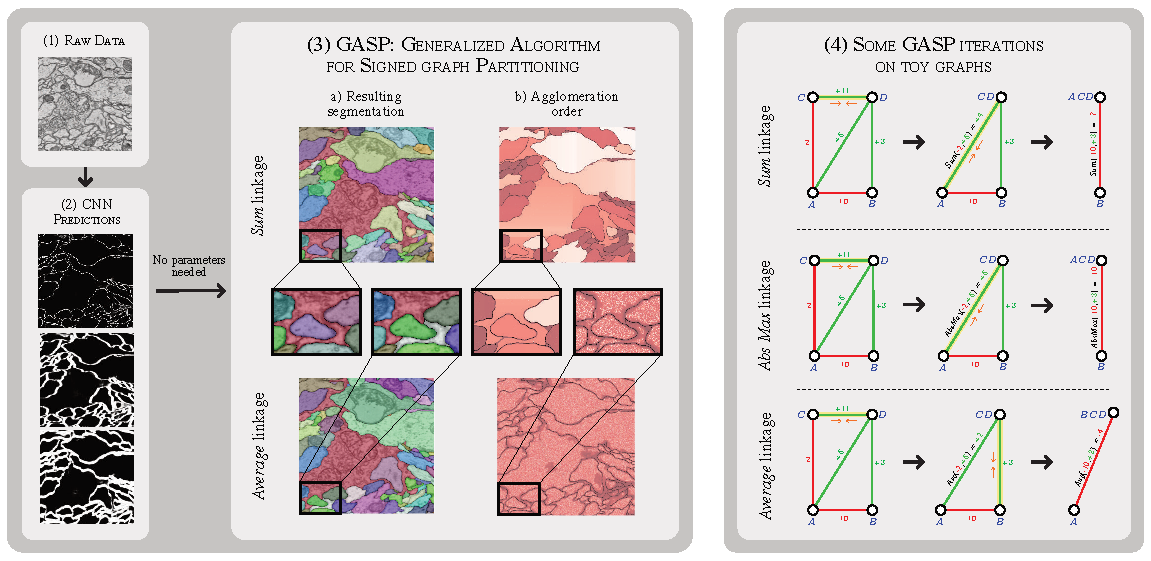
\includegraphics[width=0.5\textwidth]{figs/intro_image_v4.pdf} % left bottom right top
\caption{\TODO{Redo figure}\algname{} example. \textbf{(1)} Raw data from the CREMI 2016 neuron-segmentation challenge. \textbf{(2)} Some short- and long-range predictions of our CNN model, where white pixels represent boundary evidence. \textbf{(3)} Outputs of two agglomerative algorithms included in our proposed generalized clustering framework, with \emph{Sum} and \emph{Average} linkage criteria. The final clustering / instance segmentation is shown in 3a, overlaid with the raw image.  The  agglomeration order in 3b shows which pairs of neighboring pixels were merged first (white), later on (brown/red), or never (black). (\textbf{4}) Some iterations of \algname{} on toy graph examples with attractive/positive (green) and repulsive/negative (red) interactions. At each iteration, the yellow edge with highest interaction is contracted (orange arrows), until only negative edges are left in the graph. \TODO{Check if avg is correct}
\label{fig:intro_figure}}
\end{figure*}

\begin{table*}[t]
    \centering
    \footnotesize
    \begin{subtable}[t!]{\textwidth}\centering
        \begin{tabular}{l |c  c  c  c  c}
        % \multicolumn{1}{c}{}
        % \multirow{2}{*}[-0.5em]{\thead{\textbf{\algname{} linkage criteria} \\ $\,\,\interact(S_u ,S_v)$}}  
        & \thead{Sum\\Linkage} & \thead{Absolute Maximum\\Linkage} & \thead{Average\\Linkage} & \thead{Single\\Linkage} & \thead{Complete\\Linkage} \\
 % \multicolumn{1}{c}{} 
 & $\displaystyle \sum_{e\in E_{ij}} \cost_e$  & $\displaystyle \cost_e$ with $\displaystyle e = \argmax_{t\in E_{ij}} |\cost_t|$ & $\displaystyle \sum_{e\in E_{ij}} \cost_e \bigg/ \big|E_{ij}\big| $ &  $\displaystyle \max_{e\in E_{ij}} \cost_e$ & $\displaystyle \min_{e\in E_{ij}} \cost_e$ \\ \midrule
 % \cmidrule{2-6}

            \thead[r]{GASP on positive-weighted graphs} & \thead{-} &\thead{\textbf{HC-Single}} &\thead{\textbf{HC-Avg}} &\thead{\textbf{HC-Single}} &\thead{\textbf{HC-Complete}} \\
            \thead[r]{GASP on signed graphs} & \thead{GAEC \cite{keuper2015efficient}} & \thead{\textbf{Mutex Watershed} \cite{wolf2018mutex}}& \thead{\textbf{HC-Avg}} &\thead{\textbf{HC-Single}} &\thead{\textbf{HC-Complete}} \\
            \thead[r]{GASP on signed graphs + constraints} & \thead{\colorbox{yellow}{HCC-Sum}} % \thead{Greedy Fixation \cite{levinkov2017comparative}} 
            & \thead{\textbf{Mutex Watershed} \cite{wolf2018mutex}}& \thead{\colorbox{yellow}{HCC-Avg}} &  \thead{\colorbox{yellow}{HCC-Single}} &  \thead{\colorbox{yellow}{HCC-Complete}} \\
            % \multicolumn{2}{c|}{\multirow{2}{*}[-0.5em]{\thead{\textbf{\algname{} linkage criteria} $\,\,\interact(S_u ,S_v)$}}}  & \multirow{2}{*}[-0.5em]{\thead{\textbf{Unsigned Graphs}}} & \multicolumn{2}{c}{\thead{\textbf{Signed Graphs}}}  \\        
            % \multicolumn{2}{c|}{} &  &  \multicolumn{1}{c}{\thead{No Constraints}} & \thead{With Constraints} \\ \midrule
             

            %  Sum: & $\displaystyle \sum_{e\in E_{uv}} \cost_e$ & \thead{Sum Linkage\\Hier. Aggl. Clust.} & \thead{GAEC \cite{keuper2015efficient}} & \thead{Greedy\\Fixation \cite{levinkov2017comparative}} \\ 
            
             


            %  \makecell[r]{Abs. Max:} & 
            % $\displaystyle \cost_e$ with $\displaystyle e = \argmax_{t\in E_{uv}} |\cost_t|$
            %    & \thead{Single Linkage\\Hier. Aggl. Clust.} & \thead{Mutex\\Watershed \cite{wolf2018mutex}} & \thead{Mutex\\Watershed \cite{wolf2018mutex}} \\
             


            %  \makecell[r]{Average:} & $\displaystyle \sum_{e\in E_{uv}} \cost_e \bigg/ \big|E_{uv}\big|  $ & \thead{ Average Linkage\\ Hier. Aggl. Clust.} & \thead{\textbf{NEW}} & \thead{\textbf{NEW}}\\ 

            % Max: & $\displaystyle \max_{e\in E_{uv}} \cost_e$ & \thead{Single Linkage\\Hier. Aggl. Clust.} & \thead{\textbf{NEW}} & \thead{\textbf{NEW}}\\ 

            % Min:& $\displaystyle \min_{e\in E_{uv}} \cost_e$ & \thead{Complete Linkage\\ Hier. Aggl. Clust.}  & \thead{\textbf{NEW}} & \thead{\textbf{NEW}}

        \end{tabular}
    \end{subtable} 
    \caption{Clustering algorithms included in the proposed \algname{} framework, given a linkage criterion, a type of graph (signed or unsigned) and the optional use of cannot-link constraints. New algorithms are highlighted in yellow. Algorithms typeset in bold font define an ultrametric on the graph (see Eq.~\ref{eq:UM_def}). Algorithms included in the green box, are weight-shift invariant (see Prop.~\ref{prop:weight_shift_invariant}). 
    We denote as $E_{ij}=(S_i \times S_{j}) \cap E$ the set of edges connecting two cluster $S_i, S_j$. } 
    \label{tab:linkage-criteria}
\end{table*}


With our comparison experiments, performed both on 2D urban scenes from the CityScapes dataset and 3D electron microscopy image volumes of neurons, we benchmark all algorithms in our framework, focusing on their efficiency, robustness and tendency to over- or under-cluster.
We show that one of the new algorithms derived from our framework, based on an average linkage criterion, outperforms all previously known agglomeration methods expressed in the framework and that
it achieves competitive performance on CityScapes and the challenging CREMI 2016 segmentation benchmark.

In Sec.~\ref{sec:spectral_clust}, we also show how \algname{} outperforms spectral clustering methods on the task of neuron segmentation and how on synthetic graphs it achieves similar scores to a recently proposed spectral method for signed graphs. \TODO{Define HC and AC abbrv}

% Our code is available at \url{https://github.com/abailoni/GASP}.


